\begin{pastexam}[label={px:ncku-112-prog-02}]{成大資訊聯招 112 學年度 第 2 題}
（複選）

{[5\%]} The following graph is a maximum heap. After removing the maximum element, which of the
followings is (are) true?

\begin{center}
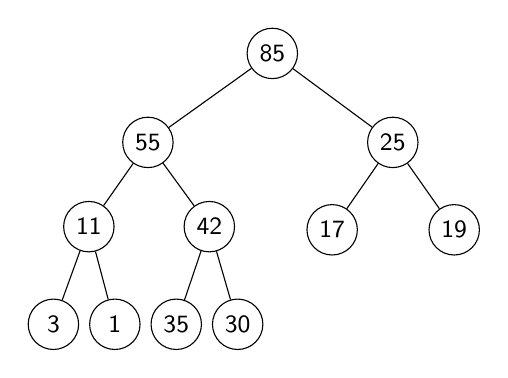
\begin{tikzpicture}[x=1cm,y=1cm,every node/.style={circle,draw,inner sep=0pt,minimum size=6.4mm,font=\sffamily\small}]
\node (n85) at (0,0) {85};
\node (n55) at (-1.58,-1.13) {55};
\node (n25) at (1.53,-1.13) {25};
\node (n11) at (-2.33,-2.2) {11};
\node (n42) at (-0.8,-2.2) {42};
\node (n17) at (0.76,-2.24) {17};
\node (n19) at (2.31,-2.24) {19};
\node (n3) at (-2.78,-3.44) {3};
\node (n1) at (-2.0,-3.44) {1};
\node (n35) at (-1.22,-3.44) {35};
\node (n30) at (-0.44,-3.44) {30};
\draw (n85)--(n55) (n85)--(n25) (n55)--(n11) (n55)--(n42) (n25)--(n17) (n25)--(n19)
      (n11)--(n3) (n11)--(n1) (n42)--(n35) (n42)--(n30);
\end{tikzpicture}
\end{center}
\begin{enumerate}[label=(\Alph*)]
\item 30 is a leaf node in the resultant heap after removal.
\item Suppose we use an array to implement the heap. The 5$^{\text{th}}$ element in the array is 30.
\item In the post-order traversal, 55 is before 42.
\item 25 is at same indexing position in the array for the post-order and in-order traversals.
\item The complexity of removal is O(log n), where n is the number of data items in the heap.
\end{enumerate}
\end{pastexam}

\begin{pastsoln}
答案：(A)(D)(E)。

\textbf{刪除最大值}（資結書第~8.1~節）。 陣列（從 $1$ 開始）是
$[85, 55, 25, 11, 42, 17, 19, 3, 1, 35, 30]$。 拿走根 $85$，把最後一個 $30$ 移到根，堆積剩 $10$ 個，
再往下調：
\begin{itemize}
\item 位置 $1$ 的 $30$，子節點 $55$、$25$，和較大的 $55$ 交換。
\item 位置 $2$ 的 $30$，子節點 $11$、$42$，和 $42$ 交換。
\item 位置 $5$ 的 $30$，子節點只有位置 $10$ 的 $35$，$35 > 30$，交換。 位置 $10$ 沒有子節點，停。
\end{itemize}
結果陣列 $[55, 42, 25, 11, 35, 17, 19, 3, 1, 30]$：
\begin{center}
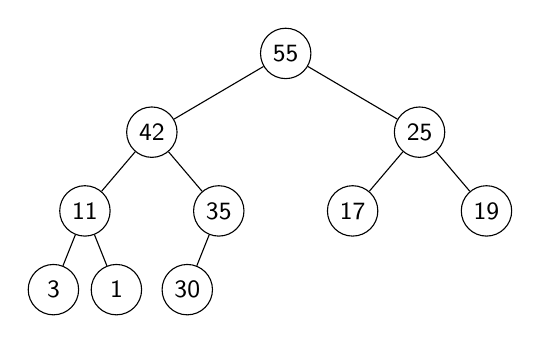
\begin{tikzpicture}[level distance=10mm,
  every node/.style={circle,draw,inner sep=0pt,minimum size=6.4mm,font=\sffamily\small},
  level 1/.style={sibling distance=34mm}, level 2/.style={sibling distance=17mm},
  level 3/.style={sibling distance=8mm}]
\node {55}
  child {node {42}
    child {node {11} child {node {3}} child {node {1}}}
    child {node {35} child {node {30}} child[missing]}}
  child {node {25} child {node {17}} child {node {19}}};
\end{tikzpicture}
\end{center}
後序：$3, 1, 11, 30, 35, 42, 17, 19, 25, 55$。 中序：$3, 11, 1, 42, 30, 35, 55, 17, 25, 19$。

逐項檢查：
\begin{itemize}
\item (A) 對。 $30$ 在位置 $10$，$2 \cdot 10 > 10$，沒有子節點，是葉節點。
\item (B) 錯。 第 $5$ 個是 $35$；$30$ 在第 $10$ 個。
\item (C) 錯。 後序先走完子樹才輪到根，$55$ 是根，排在最後；$42$ 在它的左子樹裡，比 $55$ 早。
\item (D) 對。 把兩種走訪的結果各寫成一個陣列，$25$ 在後序是第 $9$ 個，在中序也是第 $9$ 個。
\item (E) 對。 刪除只做一次往下調，最多走樹高 $\lfloor \lg n \rfloor$ 層，每層比兩次、換一次，$O(\log n)$。
\end{itemize}
\end{pastsoln}
